\documentclass[main.tex]{subfiles}
\newcommand\chapterlabel{Ch-acidbase}\setcounter{figurenewcounter}{0}\setcounter{tablenewcounter}{0}\setcounter{formulanewcounter}{0}\chapterpicture{../{\chapterlabel}/figure1}\chapterpicturelabel{PngImg}
 
\begin{document} 
\setdoublesep{0.35700 em}  % 'Bond Spacing'
\setatomsep{1.78500 em}    % 'Fixed Length'
\setbondoffset{0.18265 em} % 'Margin Width'
\renewcommand{\bondwidth}{0.06642 em} % 'Line Width'
\setbondstyle{line width = \bondwidth}

%\setcounter{chapter}{7}


  \providetoggle{chem121}\settoggle{chem121}{\chemversionhealthalied}\iftoggle{chem121}{}{
 \setcounter{chapter}{4}\import{../\chapterlabel/files/}{ChapterName}  
}
 \providetoggle{chem121}\settoggle{chem121}{\chemversionhealthalied}\iftoggle{chem121}{
 \setcounter{chapter}{9} \import{../\chapterlabel/files/}{ChapterName}  
}{}  



%       \begin{marginfigure}
%\begin{tikzpicture} \node (a) at (0,0) {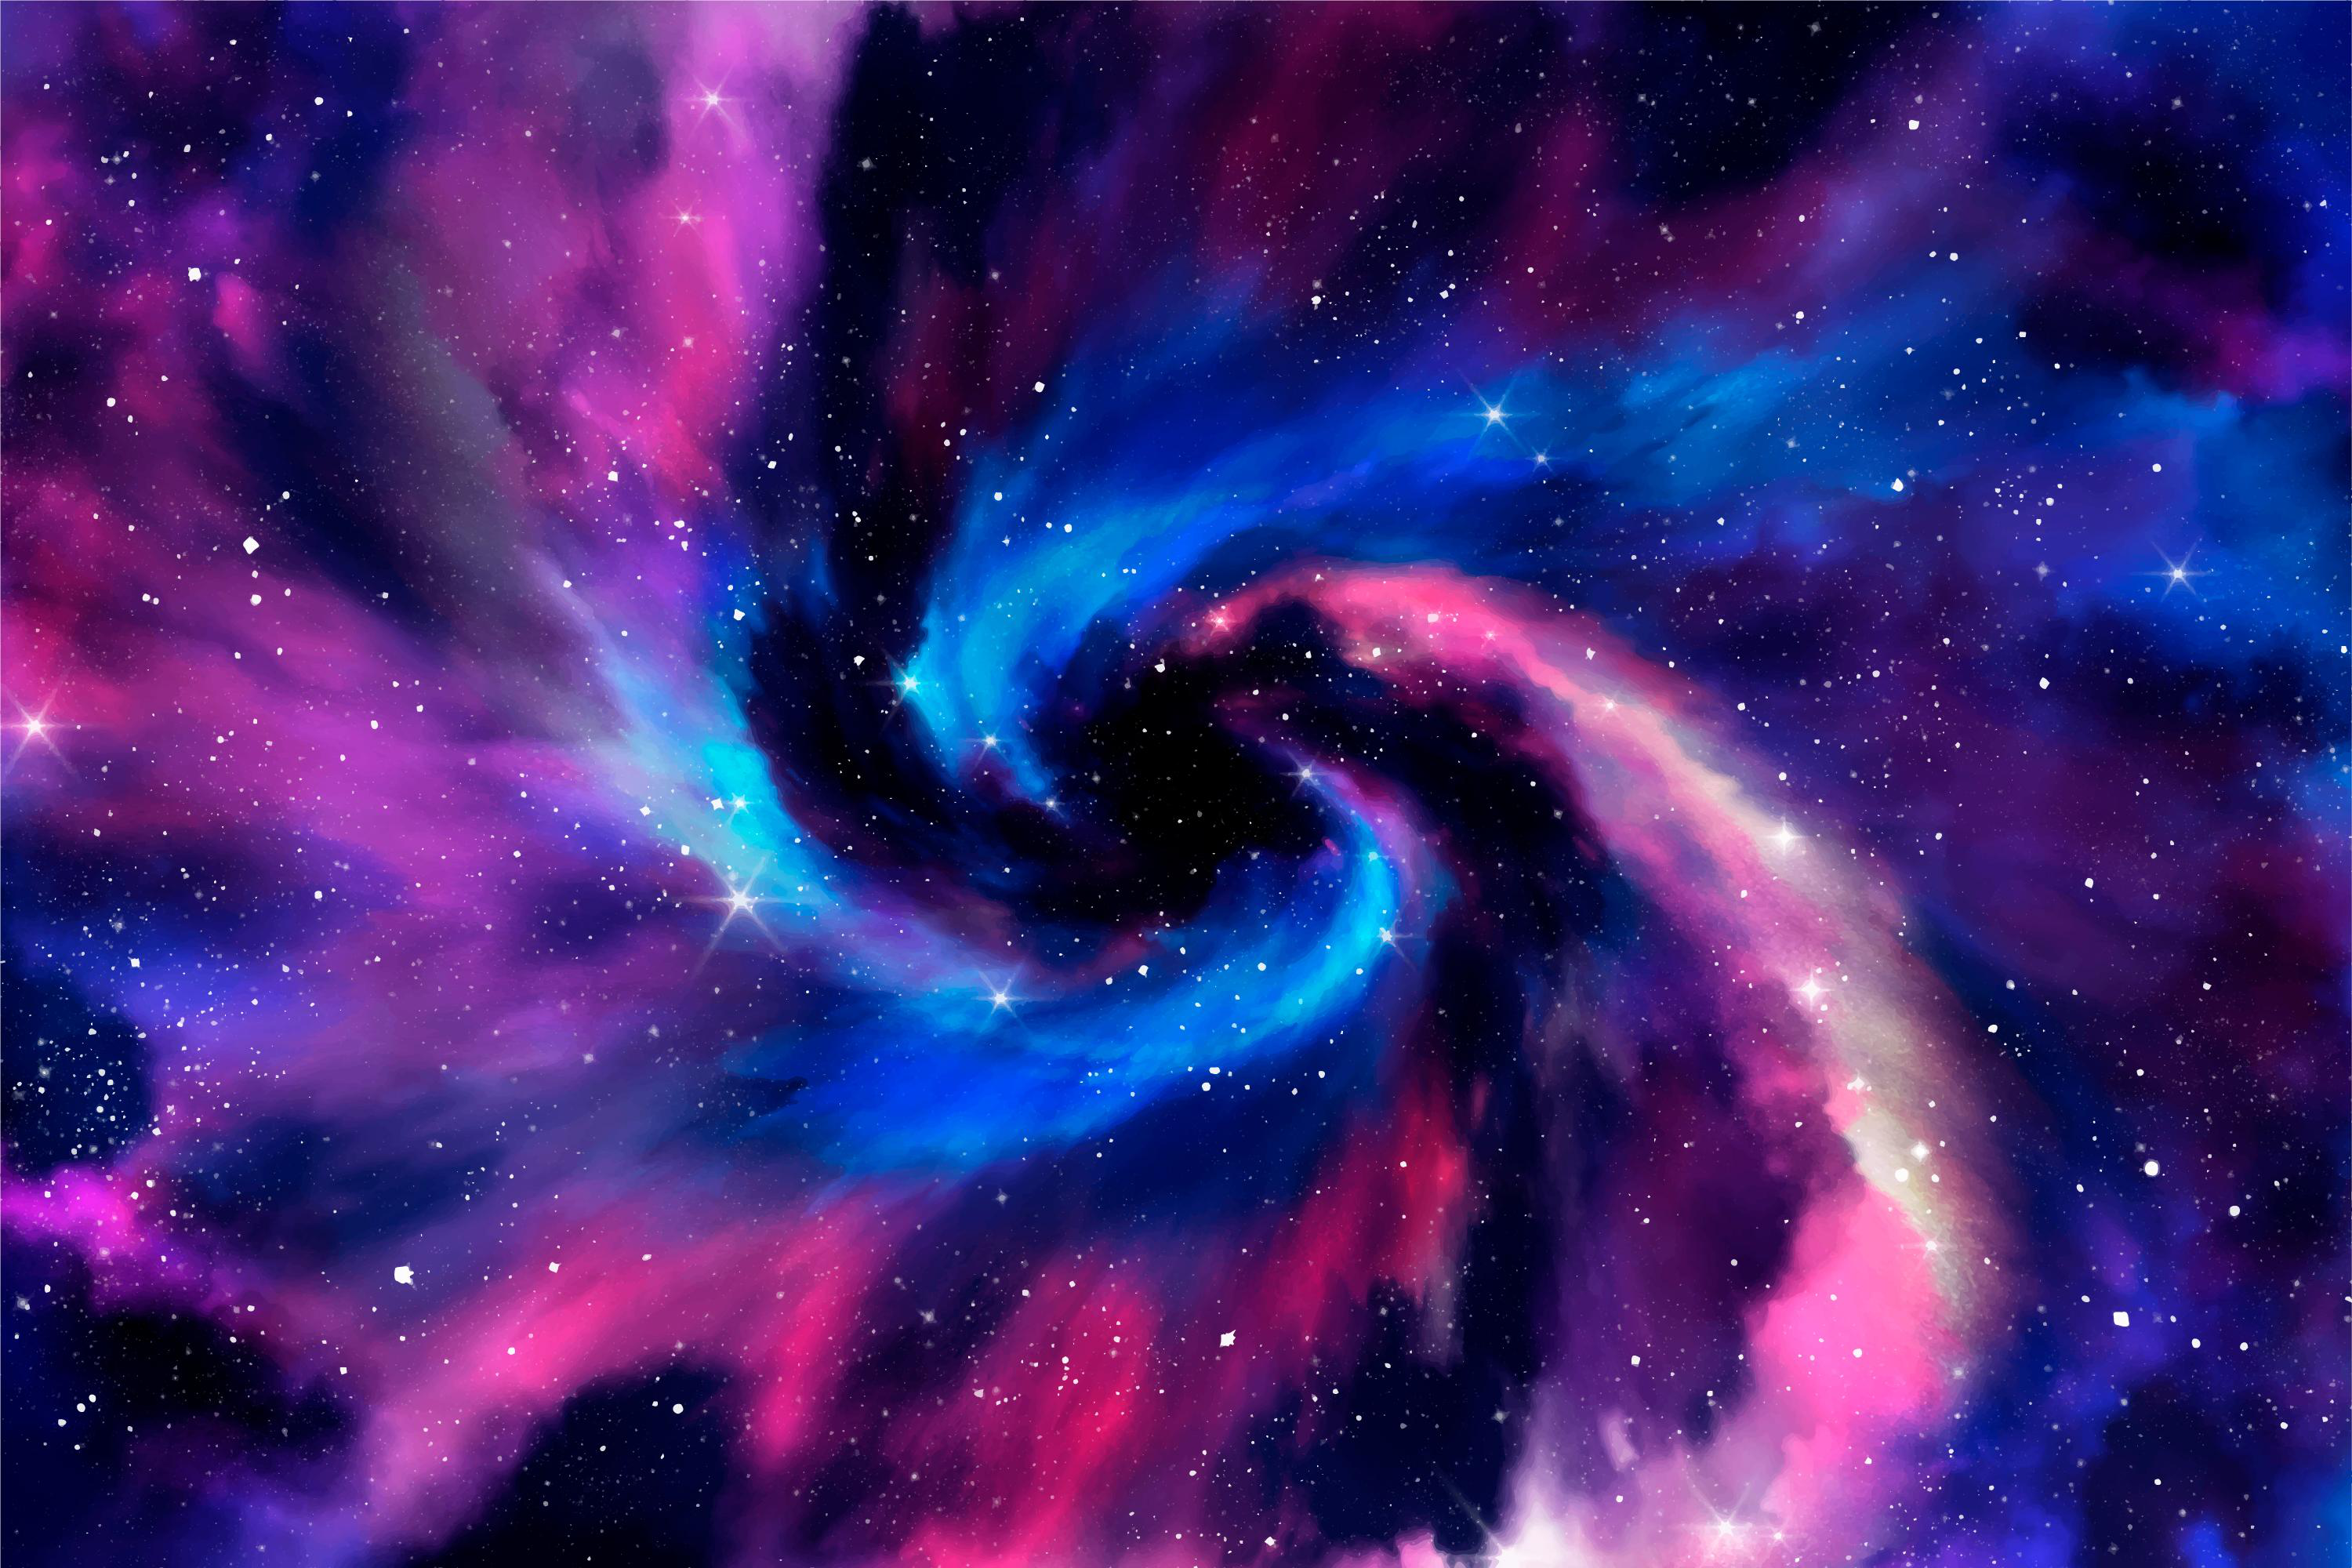
\includegraphics[width=4cm]{../Ch-acidbase/figure1}} node[rotate=90, font=\tiny] at ([yshift=.5cm,xshift=.1cm]a.south east) {\textsuperscript{\textcopyright} PngImg} ;
%\end{tikzpicture}
%\end{marginfigure}
   
  \import{../\chapterlabel/files/}{ChapterIntro}

%\begin{marginfigure}%LEARNING GOALS BOX
%\begin{mytcbox}{GOALS}
%\begin{enumerate}[label=\protect\circled{\color{white}\arabic*}]
%
%\import{../\chapterlabel/files/}{SectionGoal-Dissociation-of-acids-and-bases}
%\import{../\chapterlabel/files/}{SectionGoal-Dissociation-of-acids-and-base-Conjugate-organic-acids-and-bases}
%
%\import{../\chapterlabel/files/}{SectionGoal-Strength-of-acids-and-bases}
%\import{../\chapterlabel/files/}{SectionGoal-The-PH-scale}
%\import{../\chapterlabel/files/}{SectionGoal-Titrations}
%\import{../\chapterlabel/files/}{SectionGoal-Buffer-solutions}
%
%\end{enumerate}
%\end{mytcbox}
%\vspace{1cm}
%\begin{tcolorbox}[enhanced,colback=red!5!white,colframe=black!50!red,boxrule=1pt,
%  arc=0pt,outer arc=0pt,drop heavy lifted shadow]
%\faGears\ 
%\docenvdef{Discussion:}   \import{../\chapterlabel/files/}{ChapterDiscussion}
%\end{tcolorbox}
%\end{marginfigure}%LEARNING GOALS BOX


\section{\color{blue!30!black}{The nature of acids and Bases}}\import{../\chapterlabel/files/}{SubSection-The-nature-of-acids-and-Bases-Acids-and-bases}
\sloppy\begin{description}
\item[\docfilehook{Strong and weak acids and bases}{}] \import{../\chapterlabel/files/}{SubSection-The-nature-of-acids-and-Bases-Strong-and-weak-acids-and-bases} 
\import{../\chapterlabel/files/}{SideFigure-Common-acids-and-bases}
\item[\docfilehook{Arrhenius acid-base model}{}] \import{../\chapterlabel/files/}{SubSection-The-nature-of-acids-and-Bases-Arrhenius-acid-base-model}
\item[\docfilehook{Br\"{o}nsted-Lowry  acid-base model}{}]\import{../\chapterlabel/files/}{SubSection-The-nature-of-acids-and-Bases-Bronsted-acids}
\import{../\chapterlabel/problems/}{SampleProblem1}
\import{../\chapterlabel/files/}{SideFigure-More-common-acids}
\providetoggle{chem121}\settoggle{chem121}{\chemversionhealthalied}\iftoggle{chem121}{}{
%%%%%%%%%%%%%%%%%%%%%%NOT FOR 121
\item[\docfilehook{Lewis acid-base model}{}]\import{../\chapterlabel/files/}{SubSection-The-nature-of-acids-and-Bases-Lewis-acid-base-model} 
\import{../\chapterlabel/problems/}{SampleProblem2} 
\import{../\chapterlabel/files/}{SubSection-The-nature-of-acids-and-Bases-Acids-models-sumary}  
\begin{center} \import{../\chapterlabel/files/}{Table-Acid-models}\end{center} 
%%%%%%%%%%%%%%%%%%%%%%NOT FOR 121
}
\end{description}

\section{\color{blue!30!black}{Dissociation of acids and bases}}\import{../\chapterlabel/files/}{SectionIntro-Dissociation-of-acids-and-bases}
\sloppy\begin{description}
\item[\docfilehook{ Conjugate acids and bases}{ }] \import{../\chapterlabel/files/}{SubSection-Dissociation-of-acids-and-bases-Conjugate-acids-and-bases}
\import{../\chapterlabel/problems/}{SampleProblem3}
\item[\docfilehook{ Writing down acid-base equilibria}{ }] \import{../\chapterlabel/files/}{SubSection-Dissociation-of-acids-and-bases-Writing-down-acid-base-equilibria}
\item[\docfilehook{Including water in the dissociation}{}] \import{../\chapterlabel/files/}{SubSection-Strength-of-acids-and-bases-Including-water-in-the-dissociation}
\import{../\chapterlabel/problems/}{SampleProblem7}
\providetoggle{chem121}\settoggle{chem121}{\chemversionhealthalied}\iftoggle{chem121}{}{
%%%%%%%%%%%%%%%%%%%%%%NOT FOR 121
\item[\docfilehook{ Conjugate organic acids and bases}{ }] \import{../\chapterlabel/files/}{SubSection-Dissociation-of-acids-and-bases-Conjugate-organic-acids-and-bases} 
\import{../\chapterlabel/problems/}{SampleProblem4} 
\item[\docfilehook{Dissociating organic acids and bases}{}] \import{../\chapterlabel/files/}{SubSection-Dissociation-of-acids-and-bases-Dissociating-organic-acids-and-bases} 
\import{../\chapterlabel/problems/}{SampleProblem5} 
%%%%%%%%%%%%%%%%%%%%%%NOT FOR 121
}
\end{description}


\section{\color{blue!30!black}{Strength of acids and bases}}\import{../\chapterlabel/files/}{SectionIntro-Strength-of-acids-and-bases}
\sloppy\begin{description}
\item[\docfilehook{ Review of acid-base strength}{}] \import{../\chapterlabel/files/}{SubSection-Strength-of-acids-and-bases-Review-of-Strength}
\item[\docfilehook{ Strength of acids and bases}{}] \import{../\chapterlabel/files/}{SubSection-Strength-of-acids-and-bases-Strength-of-acids-and-bases-}
\item[\docfilehook{ Basicity constant}{}] \import{../\chapterlabel/files/}{SubSection-Strength-of-acids-and-bases-Strength-of-acids-and-bases-Basicity-constant}
\item[\docfilehook{ $K_a$ and $K_b$}{}] \import{../\chapterlabel/files/}{SubSection-Strength-of-acids-and-bases-Ka-and-Kb}
\import{../\chapterlabel/files/}{Table-Acidity-constants}
\import{../\chapterlabel/problems/}{SampleProblem6}
\item[\docfilehook{$pK_a$ and $pK_b$}{}] \import{../\chapterlabel/files/}{SubSection-Strength-of-acids-and-bases-PK-of-an-acid-or-base}
\item[\docfilehook{The conjugate seesaw}{}] \import{../\chapterlabel/files/}{SubSection-Strength-of-acids-and-bases-Conjugate-Seesaw}
\import{../\chapterlabel/files/}{SideFigure-PH-meter-and-indicators}
\providetoggle{chem121}\settoggle{chem121}{\chemversionhealthalied}\iftoggle{chem121}{}{
%%%%%%%%%%%%%%%%%%%%%%NOT FOR 121
\item[\docfilehook{Acid-base properties of salts}{}] \import{../\chapterlabel/files/}{SubSection-Strength-of-acids-and-bases-Acid-base-properties-of-salts}
\item[\docfilehook{Acid-base properties of oxides}{}] \import{../\chapterlabel/files/}{SubSection-The-nature-of-acids-and-Bases-Acid-base-properties-of-oxides}
%%%%%%%%%%%%%%%%%%%%%%NOT FOR 121
}
\end{description}


\section{\color{blue!30!black}{The PH scale}}\import{../\chapterlabel/files/}{SectionIntro-The-PH-scale}
\sloppy\begin{description}
\item[\docfilehook{ Autoprotolysis of water and $K_w$}{}] \import{../\chapterlabel/files/}{SubSection-The-PH-scale-Kw}
\item[\docfilehook{ Protons and Hydroxyls}{}] \import{../\chapterlabel/files/}{SubSection-The-PH-scale-Protons-and-Hydroxyls}
\import{../\chapterlabel/problems/}{SampleProblem8}
\item[\docfilehook{ The PH scale}{}] \import{../\chapterlabel/files/}{SubSection-The-PH-scale-The-PH-scale}
\import{../\chapterlabel/files/}{Figure-PH-scale}
\import{../\chapterlabel/problems/}{SampleProblem9}
\item[\docfilehook{ From PH to proton concentration}{}] \import{../\chapterlabel/files/}{SubSection-The-PH-scale-From-PH-to-proton-concentration}
\import{../\chapterlabel/problems/}{SampleProblem10}
\import{../\chapterlabel/files/}{Figure-PH-POH-formulas}
\end{description}

\providetoggle{chem121}\settoggle{chem121}{\chemversionhealthalied}\iftoggle{chem121}{}{
%%%%%%%%%%%%%%%%%%%%%%NOT FOR 121
\section{\color{blue!30!black}{PH of strong acid-base solutions}}  
\import{../\chapterlabel/files/}{SubSection-The-PH-scale-PH-of-strong-electrolyte-solutions} 
\import{../\chapterlabel/problems/}{SampleProblem11} 
 %%%%%%%%%%%%%%%%%%%%%%NOT FOR 121


%%%%%%%%%%%%%%%%%%%%%%NOT FOR 121
\section{\color{blue!30!black}{PH of weak acid-base solutions}}  
\sloppy\begin{description}
\item[\docfilehook{ PH of solutions of weak acids and bases}{}] \import{../\chapterlabel/files/}{SubSection-The-PH-scale-PH-of-solutions-of-weak-acids-and-bases} 
\import{../\chapterlabel/problems/}{SampleProblem12} 
\item[\docfilehook{ PH of salt solutions}{}] \import{../\chapterlabel/files/}{SubSection-The-PH-scale-PH-of-salt-solutions} 
\import{../\chapterlabel/problems/}{SampleProblem13} 
\item[\docfilehook{ Percent dissociation of weak acids and bases}{}] \import{../\chapterlabel/files/}{SubSection-The-PH-scale-Percent-dissociation-of-weak-acids-and-bases} 
\import{../\chapterlabel/problems/}{SampleProblem14} 
\end{description}
%%%%%%%%%%%%%%%%%%%%%%NOT FOR 121
}

\section{\color{blue!30!black}{Buffer solutions}}\import{../\chapterlabel/files/}{SectionIntro-Buffer-solutions}
\sloppy\begin{description}
\item[\docfilehook{ Buffers}{}] \import{../\chapterlabel/files/}{SubSection-Buffer-solutions-Buffers}
\item[\docfilehook{ PH of a Buffer solution}{}] \import{../\chapterlabel/files/}{SubSection-Buffer-solutions-PH-of-a-Buffer-solution}
\import{../\chapterlabel/problems/}{SampleProblem15}

\providetoggle{chem121}\settoggle{chem121}{\chemversionhealthalied}\iftoggle{chem121}{}{
%%%%%%%%%%%%%%%%%%%%%%NOT FOR 121
\item[\docfilehook{ PH of Buffer solution mixed with acids or bases}{}] \import{../\chapterlabel/files/}{SubSection-Buffer-solutions-PH-of-Buffer-solution-mixed-with-acids-or-bases} %%%HERE TO UP
\import{../\chapterlabel/problems/}{SampleProblem16}  
%%%%%%%%%%%%%%%%%%%%%%NOT FOR 121
}
\end{description}






\section{\color{blue!30!black}{Titrations}}\import{../\chapterlabel/files/}{SectionIntro-Titrations}
\sloppy\begin{description}
\item[\docfilehook{ Neutralization Reactions}{}] \import{../\chapterlabel/files/}{SubSection-Titrations-Neutralization-Reactions}
\item[\docfilehook{ Endpoint formula}{}] \import{../\chapterlabel/files/}{SubSection-Titrations-Endpoint-formula}
\import{../\chapterlabel/problems/}{SampleProblem17}
%%%%%%%%%%%%%%%%%%%%%%NOT FOR 121
\providetoggle{chem121}\settoggle{chem121}{\chemversionhealthalied}\iftoggle{chem121}{}{
\item[\docfilehook{ The mid-point}{}] \import{../\chapterlabel/files/}{SubSection-Titrations-Mid-point}	
}
%%%%%%%%%%%%%%%%%%%%%%NOT FOR 121

\end{description}

\providetoggle{chem121}\settoggle{chem121}{\chemversionhealthalied}\iftoggle{chem121}{}{
%%%%%%%%%%%%%%%%%%%%%%NOT FOR 121
\section{\color{blue!30!black}{Titrations curves}}\import{../\chapterlabel/files/}{SectionIntro-Titration-curves} 
\import{../\chapterlabel/files/}{Figure-Titration-curves} 
\sloppy\begin{description} 
\item[\docfilehook{ Titration curve differences}{}]\import{../\chapterlabel/files/}{SubSection-Titrations-Titration-curves-shape} 
\hspace{-5cm}\import{../\chapterlabel/files/}{Table-Titration-formulas} 
\end{description} 
%%%%%%%%%%%%%%%%%%%%%%NOT FOR 121

%%%%%%%%%%%%%%%%%%%%%%NOT FOR 121
\section{\color{blue!30!black}{Quantitative analysis of a titration}}\import{../\chapterlabel/files/}{SectionIntro-Quantitative-analysis-of-a-titration}
\sloppy\begin{description}
\item[\docfilehook{ Titration PH formulas}{}] \import{../\chapterlabel/files/}{SubSection-Titrations-Titration-PH-formulas}
\item[\docfilehook{ $c_R$ and $c_F$}{}] \import{../\chapterlabel/files/}{SubSection-Titrations-c_R-and-c_F}
\import{../\chapterlabel/problems/}{SampleProblem18}
\item[\docfilehook{ PH at the midpoint}{}] \import{../\chapterlabel/files/}{SubSection-Titrations-Midpoint}
\import{../\chapterlabel/problems/}{SampleProblem19}
\import{../\chapterlabel/files/}{Figure-Titration}
\end{description}
%%%%%%%%%%%%%%%%%%%%%%NOT FOR 121
}
 
\section{\color{blue!30!black}{Blood as a buffer}}\import{../\chapterlabel/files/}{SectionIntro-Blood-as-a-buffer}
\sloppy\begin{description}
\item[\docfilehook{ Carbon dioxide is an acid}{}] \import{../\chapterlabel/files/}{SubSection-Blood-as-a-buffer-Carbon-dioxide-is-an-acid}
\item[\docfilehook{ The dangerous change in blood PH}{}] \import{../\chapterlabel/files/}{SubSection-Blood-as-a-buffer-The-dangerous-change-in-blood-PH}
\import{../\chapterlabel/files/}{Figure-Alkalosis-and-PH}
\item[\docfilehook{ Alkalosis and carbon dioxide}{}] \import{../\chapterlabel/files/}{SubSection-Blood-as-a-buffer-Alkalosis-and-carbon-dioxide}
\import{../\chapterlabel/problems/}{SampleProblem20}
\end{description}
 
 \providetoggle{chem121}\settoggle{chem121}{\chemversionhealthalied}\iftoggle{chem121}{}{
 %%%%%%%%%%%%%%%%%%%%%%NOT FOR 121
\section{\color{blue!30!black}{Molecular mechanisms behind acid-base strength}}\import{../\chapterlabel/files/}{SectionIntro-Strength-of-acids-and-its-structure}
\sloppy\begin{description}
\item[\docfilehook{ Binary acids}{}] \import{../\chapterlabel/files/}{Subsection-Strength-of-acids-and-its-structure-Binary-Acids}
\item[\docfilehook{ Oxoacids}{}] \import{../\chapterlabel/files/}{Subsection-Strength-of-acids-and-its-structure-Oxoacids}
\item[\docfilehook{Carboxylic acids}{}] \import{../\chapterlabel/files/}{Subsection-Strength-of-acids-and-its-structure-Carboxylic-acids}
\item[\docfilehook{Molecular mechanisms behind acid-base strength: a review}{}] \import{../\chapterlabel/files/}{Subsection-Strength-of-acids-and-its-structure-review}
 \end{description}
%%%%%%%%%%%%%%%%%%%%%%NOT FOR 121

%%%%%%%%%%%%%%%%%%%%%%NOT FOR 121
\section{\color{blue!30!black}{Indicators}}\import{../\chapterlabel/files/}{SectionIntro-Indicators}
\hspace{10cm} \import{../\chapterlabel/files/}{Table-Indicators} 

\sloppy\begin{description}
\item[\docfilehook{ How do indicators function}{}] \import{../\chapterlabel/files/}{Subsection-Indicators-How-do-they-function}
\item[\docfilehook{ Selecting an indicator}{}] \import{../\chapterlabel/files/}{Subsection-Indicators-Selecting-and-indicator}
\item[\docfilehook{ Litmus paper}{}] \import{../\chapterlabel/files/}{Subsection-Indicators-Litmus}
\import{../\chapterlabel/problems/}{SampleProblem21}
\end{description}
 %%%%%%%%%%%%%%%%%%%%%%NOT FOR 121

%%%%%%%%%%%%%%%%%%%%%%NOT FOR 121
\section{\color{blue!30!black}{Titrations of polyprotic acids}}\import{../\chapterlabel/files/}{SectionIntro-Titrations-of-polyprotic-acids}
\sloppy\begin{description}
\item[\docfilehook{ PH curves of polyprotic acids}{}] \import{../\chapterlabel/files/}{Subsection-Indicators-Titrations-of-polyprotic-acids-PH-curved-of-polyprotic-acids}
\item[\docfilehook{ End points of polyprotic acids}{}] \import{../\chapterlabel/files/}{Subsection-Indicators-Titrations-of-polyprotic-acids-End-point-of-polyprotic-acids}
 \import{../\chapterlabel/files/}{Figure-Titration-curves-polyprotic}
%   \import{../\chapterlabel/problems/}{SampleProblem21}
 \end{description}
 %%%%%%%%%%%%%%%%%%%%%%NOT FOR 121
}
 
 %%%%%%%%%%%%%%%%%%%%%%%NOT FOR 121
%%%%%%%%%%%%%%%%%%%%%%%NOT FOR 121
\checkoddpage\ifoddpage \clearpage\thispagestyle{empty}\mbox{}\clearpage \else  \fi \end{document}

